\documentclass[11pt,a4paper]{article} 
\usepackage{a4wide}
\linespread{1.25}
\usepackage{graphicx}
\usepackage{amssymb}
\usepackage{amsmath}
\usepackage{float}
\usepackage{graphicx}
\usepackage{natbib}
\usepackage{tikz}
\usepackage{caption}
\usepackage{subfig}
\usepackage[hmargin=3cm,vmargin=2cm]{geometry}
\usepackage{sidecap}
\usepackage{listings}
\usepackage{color}
\usepackage{multirow}
\thispagestyle{empty}
\usetikzlibrary{arrows}


\begin{document}

\pdfpageheight=8cm
\pdfpagewidth=16.4cm

\begin{figure}
\vspace{-1.8cm}

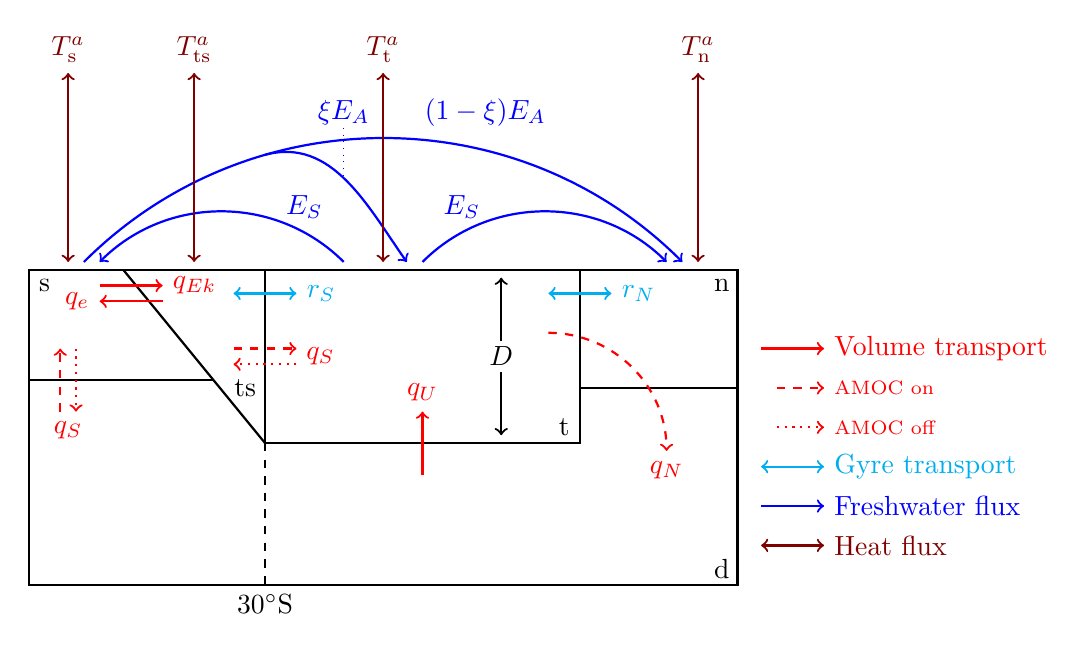
\begin{tikzpicture}[scale = 1]

\draw[thick, black] (0, 0) -- (9, 0) -- (9, 4) -- (0, 4) -- cycle;
\draw[thick, black] (3, 4) -- (3, 1.8) -- (7, 1.8) -- (7, 4);
\draw[thick, black] (7, 2.5) -- (9, 2.5);
\draw[thick, black] (3, 1.8) -- (1.2, 4);
\draw[thick, black] (0, 2.6) -- (2.34, 2.6);

\draw[black] (8.8,3.8) node {n};
\draw[black] (0.2,3.8) node {s};
\draw[black] (6.8,2) node {t};
\draw[black] (8.8,0.2) node {d};
\draw[black] (2.75,2.5) node {ts};

\draw[black] (6,2.9) node {$D$};

\draw[->, thick] (6, 2.7) -- (6, 1.9);
\draw[->, thick] (6, 3.1) -- (6, 3.9);
\draw[->, thick, red] (5, 1.4) -- (5, 2.2) node[above] {$q_U$};

\draw[->, thick, red, dashed] (2.6, 3) -- (3.4, 3);
\draw[->, thick, red, dotted] (3.4, 2.8) -- (2.6, 2.8);
\draw[red] (3.4,2.9) node[right] {$q_S$};

\draw[<->, thick, cyan] (2.6, 3.7) -- (3.4, 3.7) node[right] {$r_S$};
\draw[<->, thick, cyan] (6.6, 3.7) -- (7.4, 3.7) node[right] {$r_N$};

\draw[->, thick, red] (0.9, 3.8) -- (1.7, 3.8) node[right] {$q_{Ek}$};
\draw[->, thick, red] (1.7, 3.6) -- (0.9, 3.6) node[left] {$q_{e}$};

\draw[->, thick, red, dashed] (0.4, 2.2) -- (0.4, 3);
\draw[->, thick, red, dotted] (0.6, 3) -- (0.6, 2.2);
\draw[red] (0.5,2.2) node[below] {$q_S$};

\draw[thick, ->, red, dashed] (6.6,3.2) arc (90:0:1.5cm) node[below] {$q_N$};% syntax (starting point coordinates) arc (starting angle:ending angle:radius)

\draw[black, dashed] (3, 1.8) -- (3, 0) node[below] {30$^{\circ}$S};

\draw[blue, thick, ->] (0.7, 4.1) to [out=45,in=135] (8.3, 4.1);
\draw[blue, thick, ->] (4, 4.1) to [out=135,in=45] (0.9, 4.1);
\draw[blue, thick, ->] (5, 4.1) to [out=45,in=135] (8.1, 4.1);
\draw[blue, thick, ->] (3, 5.4605) to [out=15,in=125] (4.8, 4.1);

\draw[blue] (5.5,4.8) node {$E_S$};
\draw[blue] (3.5,4.8) node {$E_S$};
\draw[blue] (5.8,6) node {$(1-\xi) E_A$};
\draw[blue] (4,6.0) node {$\xi E_A$};
\draw[blue, dotted] (4, 5.8) -- (4, 5.2);


\draw [red!50!black, thick, <->] (0.5, 4.1) -- (0.5, 6.5) node[above] {$T_\mathrm{s}^a$};
\draw [red!50!black, thick, <->] (4.5, 4.1) -- (4.5, 6.5) node[above] {$T_\mathrm{t}^a$};
\draw [red!50!black, thick, <->] (2.1, 4.1) -- (2.1, 6.5) node[above] {$T_\mathrm{ts}^a$};
\draw [red!50!black, thick, <->] (8.5, 4.1) -- (8.5, 6.5) node[above] {$T_\mathrm{n}^a$};

\draw [red, thick, ->] (9.3, 3) -- (10.1, 3) node[right] {Volume transport};
\draw [red, thick, dashed, ->] (9.5, 2.5) -- (10.1, 2.5) node[right] {\scriptsize{AMOC on}};
\draw [red, thick, dotted, ->] (9.5, 2) -- (10.1, 2) node[right] {\scriptsize{AMOC off}};
\draw [cyan, thick, <->] (9.3, 1.5) -- (10.1, 1.5) node[right] {Gyre transport};
\draw [blue, thick, ->] (9.3, 1) -- (10.1, 1) node[right] {Freshwater flux};
\draw [red!50!black, thick, <->] (9.3, 0.5) -- (10.1, 0.5) node[right] {Heat flux};



\end{tikzpicture}
\end{figure}

$ $
\end{document}